\documentclass[border=0.2cm]{standalone}

\usepackage[scaled]{helvet}
\renewcommand\familydefault{\sfdefault}
\usepackage[T1]{fontenc}

\usepackage{tikz}
\usetikzlibrary{arrows.meta}

\definecolor{red1}{HTML}{F9665E}
\definecolor{blue1}{HTML}{A44694}
\definecolor{gold1}{HTML}{F1A226}
\definecolor{green1}{HTML}{6DDB5C}
\definecolor{purp1}{HTML}{A44694}

% Block x-offsets (adjust these to reposition entire blocks)
\newcommand{\inputX}{0}
\newcommand{\padX}{2.2}
\newcommand{\barcX}{6.1}
\newcommand{\outX}{10.0}

% Shared bar chart parameters
\newcommand{\byy}{-0.9}  % top of bar region
\newcommand{\bww}{0.35}  % bar row height
\newcommand{\bgg}{0.08}  % gap between bars
\newcommand{\barspan}{3.2} % total width of a bar chart pair

\begin{document}
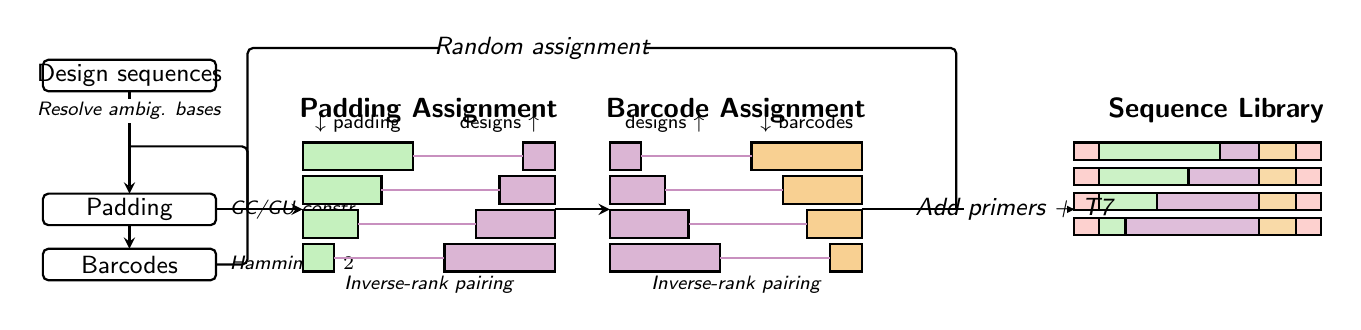
\begin{tikzpicture}

% ============================================================
% INPUTS
% ============================================================
\begin{scope}[xshift=\inputX cm]
    % Design sequences (true input)
    \draw[thick, rounded corners=2pt] (-1.1, 0.15) rectangle (1.1, -0.25);
    \node at (0, -0.05) {\small Design sequences};

    % Arrow: resolve ambiguous bases, then generate
    \draw[thick, -stealth] (0, -0.25) -- (0, -1.55);
    \draw[fill=white, draw=white] (-1.1, -0.35) rectangle (1.1, -0.65);
    \node at (0, -0.50) {\scriptsize \textit{Resolve ambig. bases}};

    % Padding
    \draw[thick, rounded corners=2pt] (-1.1, -1.55) rectangle (1.1, -1.95);
    \node at (0, -1.75) {\small Padding};
    \node[font=\scriptsize\itshape, anchor=west] at (1.15, -1.75) {GC/GU constr.};

    % Arrow
    \draw[thick, -stealth] (0, -1.95) -- (0, -2.25);

    % Barcodes
    \draw[thick, rounded corners=2pt] (-1.1, -2.25) rectangle (1.1, -2.65);
    \node at (0, -2.45) {\small Barcodes};
    \node[font=\scriptsize\itshape, anchor=west] at (1.15, -2.45) {Hamming $\geq 2$};

    % Merge designs + padding + barcodes rightward
    \draw[thick, rounded corners=2pt] (0, -0.95) -- (1.5, -0.95) -- (1.5, -1.75);
    \draw[thick]                      (1.1, -1.75) -- (1.5, -1.75);
    \draw[thick, rounded corners=2pt] (1.1, -2.45) -- (1.5, -2.45) -- (1.5, -1.75);
\end{scope}

% ============================================================
% PADDING ASSIGNMENT
% ============================================================
\begin{scope}[xshift=\padX cm]
    \node[align=center] at (1.6, -0.5) {\textbf{Padding Assignment}};

    % Padding bars (descending, left-aligned)
    \foreach \len/\i in {1.4/0, 1.0/1, 0.7/2, 0.4/3} {
        \pgfmathsetmacro{\yy}{\byy - \i*(\bww+\bgg)}
        \draw[thick, fill=green1!40] (0, \yy) rectangle ({\len}, {\yy-\bww});
    }

    % Design bars (ascending, right-aligned)
    \foreach \len/\i in {0.4/0, 0.7/1, 1.0/2, 1.4/3} {
        \pgfmathsetmacro{\yy}{\byy - \i*(\bww+\bgg)}
        \draw[thick, fill=purp1!40] ({\barspan-\len}, \yy) rectangle (\barspan, {\yy-\bww});
    }

    % Connecting lines
    \foreach \dl/\pl/\i in {1.4/0.4/0, 1.0/0.7/1, 0.7/1.0/2, 0.4/1.4/3} {
        \pgfmathsetmacro{\yy}{\byy - \i*(\bww+\bgg) - \bww/2}
        \draw[thick, purp1!60] (\dl, \yy) -- ({\barspan-\pl}, \yy);
    }

    % Labels
    \node[font=\scriptsize, anchor=south] at (0.7, \byy) {$\downarrow$ padding};
    \node[font=\scriptsize, anchor=south] at (2.5, \byy) {designs $\uparrow$};
    \node[font=\scriptsize\itshape] at (1.6, -2.70) {Inverse-rank pairing};
\end{scope}

% ============================================================
% BARCODE ASSIGNMENT
% ============================================================
\begin{scope}[xshift=\barcX cm]
    \node[align=center] at (1.6, -0.5) {\textbf{Barcode Assignment}};

    % Design bars (ascending)
    \foreach \len/\i in {0.4/0, 0.7/1, 1.0/2, 1.4/3} {
        \pgfmathsetmacro{\yy}{\byy - \i*(\bww+\bgg)}
        \draw[thick, fill=purp1!40] (0, \yy) rectangle ({\len}, {\yy-\bww});
    }

    % Barcode bars (descending)
    \foreach \len/\i in {1.4/0, 1.0/1, 0.7/2, 0.4/3} {
        \pgfmathsetmacro{\yy}{\byy - \i*(\bww+\bgg)}
        \draw[thick, fill=gold1!50] ({\barspan-\len}, \yy) rectangle (\barspan, {\yy-\bww});
    }

    % Connecting lines
    \foreach \dl/\pl/\i in {0.4/1.4/0, 0.7/1.0/1, 1.0/0.7/2, 1.4/0.4/3} {
        \pgfmathsetmacro{\yy}{\byy - \i*(\bww+\bgg) - \bww/2}
        \draw[thick, purp1!60] (\dl, \yy) -- ({\barspan-\pl}, \yy);
    }

    % Labels
    \node[font=\scriptsize, anchor=south] at (0.7, \byy) {designs $\uparrow$};
    \node[font=\scriptsize, anchor=south] at (2.5, \byy) {$\downarrow$ barcodes};
    \node[font=\scriptsize\itshape] at (1.6, -2.70) {Inverse-rank pairing};
\end{scope}

% ============================================================
% OUTPUT: stacked construct diagrams
% ============================================================
\newcommand{\outMerge}{10.5} % x where both paths merge
\newcommand{\outStart}{12.0} % x where constructs begin

\begin{scope}[xshift=\outStart cm]
    \node[align=center, font=\bfseries] at (1.8, -0.5) {Sequence Library};

    % Each construct: red flank | green pad | purple design | gold barcode | red flank
    % Real proportions: flank=20nt, design+pad=130nt, barcode=30nt, total=230nt
    % Scale: 3.6cm total width -> 1cm per ~64nt
    \def\scale{0.01565}  % cm per nt: 3.6/230
    \pgfmathsetmacro{\fw}{20*\scale}    % flank: 0.313
    \pgfmathsetmacro{\bkw}{30*\scale}   % barcode: 0.470
    \pgfmathsetmacro{\tw}{130*\scale}   % design+pad: 2.035
    \def\rh{0.22}  % row height
    \def\rg{0.10}  % row gap

    % design lengths in cm (varying, pad = tw - dw)
    \foreach \dw/\i in {0.5/0, 0.9/1, 1.3/2, 1.7/3} {
        \pgfmathsetmacro{\yy}{-0.9 - \i*(\rh+\rg)}
        \pgfmathsetmacro{\pw}{\tw - \dw}
        \pgfmathsetmacro{\x}{0}
        % 5' flank
        \draw[thick, fill=red1!30] (\x, \yy) rectangle ({\x+\fw}, {\yy-\rh});
        \pgfmathsetmacro{\x}{\x+\fw}
        % padding
        \draw[thick, fill=green1!35] (\x, \yy) rectangle ({\x+\pw}, {\yy-\rh});
        \pgfmathsetmacro{\x}{\x+\pw}
        % design
        \draw[thick, fill=purp1!35] (\x, \yy) rectangle ({\x+\dw}, {\yy-\rh});
        \pgfmathsetmacro{\x}{\x+\dw}
        % barcode
        \draw[thick, fill=gold1!40] (\x, \yy) rectangle ({\x+\bkw}, {\yy-\rh});
        \pgfmathsetmacro{\x}{\x+\bkw}
        % 3' flank
        \draw[thick, fill=red1!30] (\x, \yy) rectangle ({\x+\fw}, {\yy-\rh});
    }
\end{scope}

% ============================================================
% INTER-BLOCK ARROWS
% ============================================================

% Inputs -> Padding assignment
\draw[thick, -stealth] ({\inputX+1.5}, -1.75) -- (\padX, -1.75);

% Padding -> Barcode assignment
\draw[thick, -stealth] ({\padX+\barspan}, -1.75) -- (\barcX, -1.75);

% Barcode -> merge point
\draw[thick] ({\barcX+\barspan}, -1.75) -- (\outMerge, -1.75);

% Random path (shortcut over top, merges at same point)
\draw[thick, rounded corners=2pt]
    ({\inputX+1.5}, -1.75) -- ({\inputX+1.5}, 0.3)
    -- (\outMerge, 0.3)
    -- (\outMerge, -1.75);

\draw[fill=white, draw=white] ({(\inputX+\outMerge)/2-1.3}, 0.15) rectangle ({(\inputX+\outMerge)/2+1.3}, 0.45);
\node at ({(\inputX+\outMerge)/2}, 0.3) {\small \textit{Random assignment}};

% Merge point -> output (with inline label)
\draw[thick, -stealth] (\outMerge, -1.75) -- (\outStart, -1.75);
\draw[fill=white, draw=white] ({\outMerge+0.1}, -1.60) rectangle ({\outStart-0.1}, -1.90);
\node at ({(\outMerge+\outStart)/2}, -1.75) {\small \textit{Add primers + T7}};

\end{tikzpicture}
\end{document}
